\chapter{System Evaluation}

\subsection{Objectives Set Out}
From the outset the main objective was to create an application worthy of being a prototype system to be able demonstrate to fellow colleagues at work and companies that implement stock control systems to shops. The goal was to create an application that could tackle the existing issue of date checking not being as effective as it should be. This application will benefit staff members in saving time and stores in saving money by being able to take action early with products close to their sell by dates and also saving money in the future looking at the popularity of the product and look at the aspect of maybe saving money by not ordering a product as it didn't sell as well as it was targeted to do so.
\newline

This project from the outset was to achieve a personal objective of making an application to be proud of. That in the future can look back on what was created and feel a sense of self-achievement that this is what was created and that it can solve an existing issue linked to life outside of the college environment and into a place I have worked in for over five years. 
\newline

Conducting a survey among the staff at the workplace to get their valued opinions on this idea that will heavily involve them potentially using this in the future was a goal that could be achieved. This feedback will be very relevant to me as the developer and as it is to those that will be using the application on a daily basis. As a result of this the application needed to be very easy to use and understand. Not making it complicated to use which will cause for carelessness to use it. Making it quick and easy to use for staff is a prime objective set out from the outset. Once ready the staff will be shown a demonstration of the application to get their thoughts overall.
\newline
\newpage
Outside of the purposeful objectives I hoped to learn more and gain more insight into the technologies used throughout the project. not to mention learning more about the Ionic framework and the Firebase cloud database storage. Also Furthering my knowledge in GitHub, Visual Studio Code and Overleaf LaTeX. Beyond this project the wish is to develop more Ionic applications with the Firebase cloud storage and being more knowledgeable in the framework and database will benefit beyond college and into potential employment.  

\subsection{Objectives Met or Not Met}
With the objectives set out from the outset the majority if not all objectives set out were met to self satisfaction. There are some minor aspects in the application that might be added in the future to the application, however this is a prototype that is designed in a way to demonstrate to shops and companies who are linked to shops such as CBE. Overall I am pleased with what was produced as it is helping an area close to life outside college and knowing it will save staff the hassle of checking every product where as with this they can just see whats close or past its sell by date pinpointing what needs to be done rather than physically looking where it is possible that they might miss something which then puts the customer at risk along with the shop if something were to happen.
\newline

The main objective set out was to develop an application for to improve date checking sufficiency within the retail business and to save staff time in identifying stock close or past their sell by date. An application was successfully created that will indeed save the shop money in terms of getting to the product in time and taking action and intercept the danger of a customer purchasing and consuming an out of date product. From experience that not every customer checks the date of products and not to mention being in a scenario where a customer has actually brought up or notified me of a product passed or close to its sell by date. The regulations in the shop is to remove or reduce an item two days before its sell by date. The purpose of this application improves this and will save the staff time in a busy schedule and the shop money in using the product elsewhere or enable them to make future decisions regarding a product and the number of products found.
\newline

A survey was conducted within the workplace which was one of the objectives set out, to get a sort of second opinion on the potential implementation of this application to their daily routine. This objective was met and was crucial in the planning and development of the application, taking into account mainly those who questioned the idea and if it was necessary. The hope was to get a mixture of feedback for this which would allow me to then suss out the pros and cons of making this application and potentially using it within the workplace. All feedback was appreciated both positive and negative. 
\newline
\newpage
The ambition to learn more about the Ionic Framework and Firebase Cloud Database in which was met, which is pleasing as in the future the hope is to develop more projects using these technologies. More was learned specifically about making an application a Firebase hosting website which was a first and a sense of achievement that this application was now active and live for people to use instead of running an "ionic serve" and installing the required libraries to do so which isn't a sufficient way of application usage and demonstration so it was pleasing to learn more about this and implement this into my application. There is now a sense of easy transportation of this application rather than having to be just be on one particular device to use the application. Not to mention improving my GitHub knowledge in terms of insights and to show issues within development. I also enhanced my use of Visual Studio Code and the use of command lines. Also improving the newly learned LaTeX skills after first coming across this in the first semester of this academic year. So it is safe to say I improved my usage and skill of the technology used for development in which is very pleasing as it will benefit for future projects and tasks outside of college. 
\newline

Overall the feeling is that the Objectives and Goals set out in making an application were met, not only for its intended purpose but for a sense of self-achievement for making an application to tackle a global issue when it comes to food wastage and consumption of foods that could endanger a person. During the course of development of this project weekly goals and objectives were set out in development which was discussed with the project supervisor in our weekly meetings. This is great in terms of getting work done in a timely manner.

\subsection{Application Testing Results}
As mentioned in the Technology Review application tests were conducted for the applications functionality. To test functions such as user authentication logging in, registration and logging out. Along with adding, updating and deleting food products from their designated food group. 
\newline

Results shown on the next page:
\newpage
\begin{figure}[h!]
	\caption{Application Testing Result Page 1}
	\label{image:test1}
	\centering
	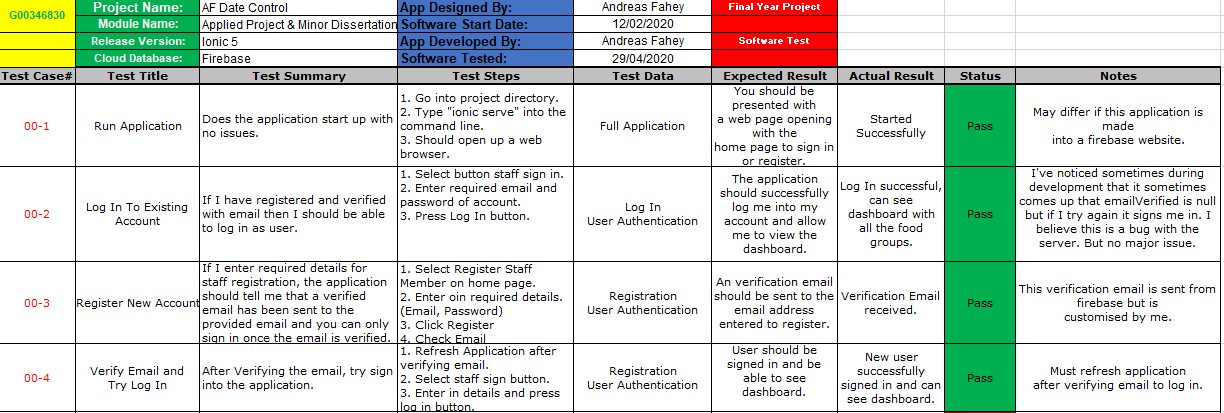
\includegraphics[width=0.9\textwidth]{images/testResults1.PNG}
\end{figure}

\begin{figure}[h!]
	\caption{Application Testing Result Page 2}
	\label{image:test2}
	\centering
	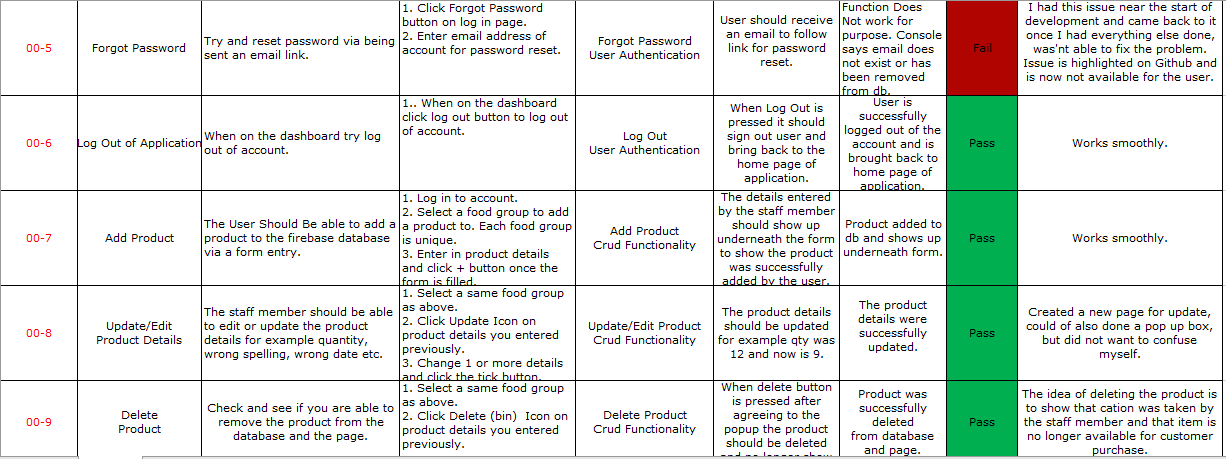
\includegraphics[width=0.9\textwidth]{images/testResults2.PNG}
\end{figure}

- Noticed when logging in a potential bug has been noted which is highlighted on the GitHub Repository where a window popup shows a an email verified null error. When canceled and clicked log in again it allows me to log in. Note if you try log in with an unverified email it will tell you so, this is a different issue but does not hinder application functionality. 
\newline

- Unfortunately it was unattainable to get the password recovery/reset function working as you can see in the test document screenshot above it failed. This is also a highlighted issue on the GitHub repository. The code is available but commented out as it was failing in the "ionic build" command for making the application a Firebase website.
\newline

- These application tests also give a sense of the know how to an application. An instruction manual if you will. Shows a tester or user how to do certain things such as register an account or update a food product for example. It of course is good in showing what does work and what doesn't when presenting this to someone. Maybe they could fix an issue or a failed test ? These application tests can be useful in more than one sense.
\newpage
\subsection{Survey Results}

\begin{figure}[h!]
	\caption{Survey Results}
	\label{image:surveyResults}
	\centering
	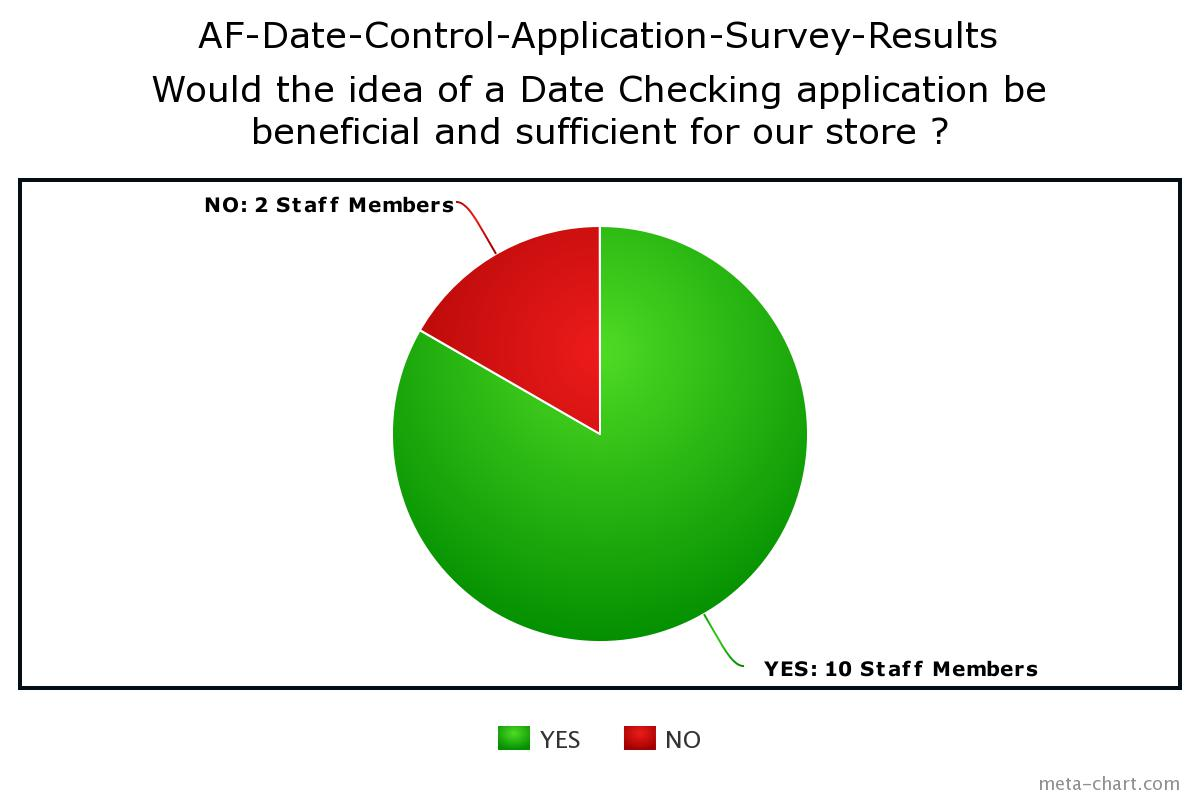
\includegraphics[width=0.9\textwidth]{images/AF-Date-Control-Survey-Results.jpeg}
\end{figure}

Above shows the results of the survey conducted into a pie chart. It shows that two thought this idea was unnecessary with one reason being "Not everyone is good with technology" and the other reason being "Not necessary, if products are checked regularly there is no need for anything extra". Feedback is appreciated and the reasoning was acknowledged. Yes I agree that not everyone is good with technology but I counter that with the fact that technology plays a major role in our lives on a daily basis be it using a computer and even a smart phone which is the norm for phone users nowadays. Technology is taking over so why be left behind. I also agree that if products are checked regularly that it will cover most of the products but not all in my opinion. This application shows exactly what is close or past its sell by date so the staff member can then find the product without having to check every single product. Also, from experience knowing that working in a shop can be very busy which gives the worker a lack of time to get things done such as date checking, as mentioned previously this reduces the time spent date checking while making it more sufficient in the grand scheme of things. 
\newpage
\subsection{Limitations}
There were some limitations in the development of this project. The major one not being able to have access to a shop database to show a full example of the purpose of this application and show what it is intended to do. In lieu of this a product entry form was added to show what it would look like in real time in a shop. Was also unable to implement product data sort by date which will make it easier for the staff members to go to the top of the list of products where they will find products closest or past their sell by dates, but the idea was there. Discussions took place about the idea of highlighting a product orange if it was two days before going out of date and red if the product is passed its best before date. Maybe in the future these aspects could be added to the application to again make it easier for staff members to use and understand. The fact that this is a prototype allows for some stuff not to be implemented as intended as long as the idea is there. Resetting the user password functionality was another aspect I was unable to implement into this application, the code is commented out as mentioned above it was throwing errors in the build for the Firebase website. Prototypes tend to have certain limitations, however personally would have liked to have had these characteristics in the application.